% Created 2019-05-23 jeu. 07:38
% Intended LaTeX compiler: pdflatex
\documentclass[11pt]{article}
\usepackage[utf8]{inputenc}
\usepackage[T1]{fontenc}
\usepackage{graphicx}
\usepackage{grffile}
\usepackage{longtable}
\usepackage{wrapfig}
\usepackage{rotating}
\usepackage[normalem]{ulem}
\usepackage{amsmath}
\usepackage{textcomp}
\usepackage{amssymb}
\usepackage{capt-of}
\usepackage{hyperref}
\usepackage{minted}
\usepackage[margin=2cm]{geometry}
\usepackage[demo]{graphicx}
\usepackage{subcaption}
\author{Thomas}
\date{\today}
\title{}
\hypersetup{
 pdfauthor={Thomas},
 pdftitle={},
 pdfkeywords={},
 pdfsubject={},
 pdfcreator={Emacs 26.1 (Org mode 9.2.3)}, 
 pdflang={English}}
\begin{document}

\tableofcontents


\section{Résumé}
\label{sec:orgddbb1cf}

Ce document présente la solution apportée par notre groupe au projet que nous à proposé CIL4SYS : utiliser l'apprentissage statistique dans le but de fluidifier le trafic en zone urbaine. Nous proposons à ce stade un modèle DQN ayant pour but de contrôler les feux tricolores sur un morceau de quartier d'Issy les Moulineaux.

\section{Introduction}
\label{sec:orge484377}

Alors que l'écologie devient un enjeu international d'importance, de plus en plus de recherches sont faites sur des transports verts, ou sur des moyens d'économiser de l'énergie. Dans le même temps, les avancées technologiques laissent présager une arrivée de véhicules autonomes capables de communiquer avec leur environnement, ou du moins de l'intelligence artificielle comme assistance de conduite. Dans ce contexte, plusieurs études ont été metnées dans le but de réduire les émissions de polluants des véhicules par l'intermédiaire de la fluidification du trafic routier. Parmi ce domaine de recherche, on distingue notamment les travaux se concentrant sur les zones extra-urbaines (autoroutes et grands axes routiers) [citer papiers sans commenter], des zones urbaines qui sont au c\{\oe\}ur du sujet traité dans ce rapport. La start-up CIL4SYS nous propose, dans le cadre d'un projet fil-rouge, de nous pencher sur la possibilité de réduire les émissions de polluants dans l'hypothèse de feux tricolores intelligents capables d'envoyer des consignes de vitesse aux véhicules traversants un quartier en zone urbaine dans le but de limiter les accélérations et décélérations des véhicules sources de fortes consommations en carburant.

Le projet s'articule donc autour de CIL4SYS créée en juin 2015 par Philippe GICQUEL qui a travaillé pendant 25 ans en R$\backslash$&D automobile chez EDAG et PSA Peugeot-Citroën. Le c\{\oe\}ur de métier de CIL4SYS étant de proposer une solution permettant de générer des cahiers des charges et des spécifications techniques à partir de diagrammes UML décrivant le fonctionnement désiré d'un système. Leur cible principale étant l'industrie automobile, un environnement de simulation a été spécifiquement développé dans le but de répondre à cette industrie. Mais aussi de SOFTEAM, grand groupe fournissant un panel de service divers, allant du consulting opérationnel et métier, à la modélisation et l'automatisation, en passant par l'innovation. Leur rôle, durant ce projet, sera de nous assister lors de la phase de machine-learning en nous apportant une expertise avancée en data science. Enfin TélécomParisTech constitue le dernier acteur de ce projet par l'intermédiaire de notre groupe d'étudiants chargé d'effectuer les premiers développements et essais ainsi que de proposer les solutions et méthodes à explorer.$\backslash$

L'objectif principal de ce projet est donc de démontrer à l’échelle d’un quartier que par un contrôle à la fois des feux tricolores et des vitesses des véhicules (dans un contexte où les véhicules sont communicants et peuvent recevoir des instructions de vitesse), il est possible de trouver un optimum de diminution des rejets de polluants et de CO2. Les méthodes mises en place au cours du projet devront faire appel à nos connaissances en apprentissage automatique afin de proposer une première approche de résolution.

Il nous est demandé de d'utiliser nos connaissances pour proposer une solution de machine learning à ce problème.

\section{Formulation d'optimisation}
\label{sec:orgd06fd0e}

Plus classiquement, il est possible de donner une formulation d'un point de vue optimisation du problème. En effet, l'objectif principal demandé par CIL4SYS est de trouver des lois de commande des feux et des véhicules de manière à réduire au maximum les émissions de CO2. Au cours de ce projets les émissions de CO2 seront modélisées uniquement par l'intermédiaire des accélérations. Une première approche peut donc être de minimiser

\begin{latex}
\begin{equation}
\min_{\theta(t)}{\mathbb{E}\left [\sum_{j=1}^{m} \int_{t = 0}^{t^{sortie}_{j}}{ | a_{j}(t,\theta(t),\mathcal{C}_{j}(\xi)) | dt} \right ]},
\end{equation}
\end{latex}

où \(a_{j}(t)\) représente les accélérations subies par le véhicule \(j\) tout au long de sa trajectoire \(\mathcal{C}_{j}\) affectée aléatoirement par la variable aléatoire \(\xi\) et \(\theta(t)\) représente la loi de commande imposée aux véhicules.

On constate d'ors et déjà que la solution à un tel problème d'optimisation est évidente puisqu'il suffit d'imposer une loi de commande de telle sorte que les véhicules restent à l'arrêts pour minimiser les emissions. Le problème initial d'optimisation se doit donc d'être complété par l'intermédiaire de contraintes afin répondre à un certain réalisme. Un première contrainte à envisager est le temps de trajet pour la réalisation du parcours \(\mathcal{C}\) du véhicule. En utilisant les données TOMTOM, il sera donc possible de déterminer au sein du quartier qui sera choisi par la suite quel est le temps de trajet moyen réalisé par un véhicule pour une trajectoire imposée \(\bar{t}(\mathcal{C})\). Une contrainte seuil sur le temps de trajet pourra alors être imposé avec pour référence le temps de trajet calculé. Le problème de minimisation se reformule alors de la manière suivante


\begin{latex}
\begin{equation}
\begin{cases}
\displaystyle{\min_{\theta(t)}{\mathbb{E}\left [\sum_{j=1}^{m} \int_{t = 0}^{t^{sortie}_{j}}{ | a_{j}(t,\theta(t),\mathcal{C}(\xi)) | dt} \right ]}}\\
\text{s.t.~} t^{sortie}_{j} \leq \alpha \cdot \bar{t}(\mathcal{C})
\end{cases}
\end{equation}
\end{latex}

La formalisation du problème d'optimisation reste à compléter et on sera amené à ajouter d'autres contraintes au cours du projet au fur et à mesure de sa prise en main. La fonction de coût à minimiser sera elle aussi amenée à être changée si par exemple le nombre de voitures qui traversent le quartier devient aléatoire lui aussi etc\ldots{}

\section{Apprentissage par renforcement}
\label{sec:orgf8c3b29}

Comme dit précédemment, une des méthodes utilisée dans la littérature actuelle pour effectuer de la fluidification de trafic est l'apprentissage par renforcement. C'est la méthode d'apprentissage sur laquelle nous avons décidée de nous concentrer car novatrice dans le domaine de l'optimisation de trafic routier. Dans cette section, nous présentons les grandes ligne de cette méthode d'apprentissage.

L'apprentissage par renforcement est une méthode statistique de prise de décision dans un environnement donné. L'environnement est modélisé par un état, et l'acteur peut réaliser une action qui affectera l'état. L'algorithme est guidé lors de la phase d'entraînement par une fonction de récompense. Après avoir pris une action \(a\) à un état \(e\), l'observation du nouvel état permet le calcul d'une récompense, \(r \in \mathbb{R}\).

Notons \(\mathcal{E}\) l'ensemble des états possibles de notre environnement, \(\mathcal{A}\) l'ensemble des actions possibles, et \(r_t\) la récompense obtenue au pas de temps \(t\). En modélisant la récompense cumulative comme un processus de Markov, elle ne dépend que de l'action prise et de l'état du système aux temps \(t \geq t_0\) et est définie de la manière suivante:

\begin{latex}
\[
R_{t_0} = \sum^\infty_{t=t_0} \gamma^{t-t_0}r_{t+1}
\]
\end{latex}

Où le coefficient \(\gamma \in [0,1]\) permet de donner plus de poids aux récompenses proches de \(t_0\) dans le temps et à la somme de converger.

Le principe de l'apprentissage par renforcement est alors de chercher une fonction \(Q^*: \mathcal{E} \times \mathcal{A} \longrightarrow \mathbb{R}\) qui estime le retour cumulatif \(R_{t_0}\) pour une action \(a \in \mathcal{A}\) réalisée à un état \(e \in \mathcal{E}\).

La fonction \(\pi(e,a)\) retourne la probabilité de réaliser une action \(a\) à l'état \(e\). Nous avons donc \(\sum_{a\in\mathcal{A}}\pi(e,a) = 1\). Définissons \(Q^\pi(e,a)\), la fonction qui prédit l'espérance de la récompense cumulative sous \(\pi\) sachant \(e\) et \(a\):


\begin{equation}
\label{eqn:q_value}
  Q^\pi(e, a) = \mathbb{E}_\pi[R_t|e_t=e,a_t=a]
\end{equation}

Définissions \(\mathcal{P}^a_{ee'}\), la probabilité de passer d'un état \(e\) à un état \(e'\) sachant un état \(e\) et une action \(a\) donnés :

\begin{latex}
\[
\mathcal{P}^a_{ee'} = \mathbb{P}(e_{t+1}=e'|e_t=e, a_t=a)
\]
\end{latex}

Définissions aussi \(\mathcal{R}^a_{ee'}\), l'espérance de la récompense \(r_{t+1}\)
sachant un état \(e\), et une action \(a\) à l'instant \(t\) ainsi qu'un état \(e'\) à
l'instant \(t+1\):

\begin{latex}
\[
\mathcal{R}^a_{ee'} = \mathbb{E}(r_{t+1}|e_t=e, e_{t+1}=e', a_t=a)
\]
\end{latex}

Il est alors possible de d'exprimer \(Q^\pi\) de la manière suivante:

\begin{latex}
\begin{align}
Q^\pi(e, a) &= \mathbb{E}_\pi[R_t|e_t=e,a_t=a] \\
&= \mathbb{E}_\pi[\sum_{t=t_0}^\infty \gamma^{t-t_0}r_t|e_{t_0}=e,a_{t_0}=a] \\
&= \mathbb{E}_\pi[r_{t+1}+\gamma\sum_{t=t_0}^\infty \gamma^{t-t_0}r_{t_0+1}|e_{t_0}=e,a_{t_0}=a] \\
&= \sum_{e'}\mathcal{P}^a_{ee'}\left[ \mathcal{R}^a_{ee'} +
  \gamma\mathbb{E}_\pi \left( \sum^\infty_{t=t_0}\gamma^{t-t_0}r_{t_0+1}|e_{t+1}=e' \right) \right] \\
&= \sum_{e'}\mathcal{P}^a_{ee'}\left[ \mathcal{R}^a_{ee'} +
  \gamma\sum_{a'}\mathbb{E}_\pi \left(
    \sum^\infty_{t=t_0}\gamma^{t-t_0}r_{t_0+1}|e_{t+1}=e', a_{t+1}=a' \right) \right] \\
&= \sum_{e'}\mathcal{P}^a_{ee'}\left[ \mathcal{R}^a_{ee'} +
  \gamma\sum_{a'} \pi(e',a')Q^\pi(e', a') \right]
\end{align}
\end{latex}

Si la politique d'action à choisir dans un état donné consiste à maximiser la
récompense cumulative, alors:

\begin{latex}
\[
\pi^*(e) = \underset{a}{\mathrm{argmax}} Q^*(e, a)
\]
\end{latex}

Cependant, nous ne connaissons pas la fonction \(Q^*\), nous utilisons donc un
modèle statistique pour l'approcher. En prenant alors:

\begin{latex}
\[
\pi(e) = \underset{a}{\mathrm{argmax}} Q^\pi(e, a)
\]
\end{latex}


L'équation de \(Q^\pi(e,a)\) sous cette politique se simplifie alors:

\begin{latex}
\[
Q^\pi(e,a) = r + \gamma Q^\pi(e', \pi(e'))
\]
\end{latex}


\subsubsection{Exploration vs exploitation}
\label{sec:org4ceccbb}

Au début de l'apprentissage, la fonction approchée par notre modèle ne sera pas de bonne qualité, et donc notre politique de prendre l'action avec la plus grande valeur de \(Q^\pi_\theta\) peut potentiellement ne pas converger. Pour encourager l'algorithme à explorer son espace d'action, on introduit un paramètre \(\epsilon \in [0,1]\). On modifie alors notre politique d'action de manière à faire une action aléatoire dans \(\epsilon\%\) des cas:

\begin{latex}
\[
\pi(e)=\begin{cases}
    \mathrm{random}(\mathcal{A}), & \text{si $\mathrm{random}([0,1])<\epsilon$}.\\
    \underset{a}{\mathrm{argmax}} Q^\pi(e, a), & \text{sinon}.
  \end{cases}
\]
\end{latex}


Il est aussi possible de faire varier \(\epsilon\) dans le temps, avec par exemple des valeurs plus grosses en début d'entraînement pour ensuite diminuer. Le Listing \ref{code:eps_greedy} propose une implémentation possible de stratégie \(\epsilon\) – greedy en Python.

\begin{listing}[htbp]
\begin{minted}[]{python}
def act(self, state):
    if np.random.rand() < self.epsilon:
        return random.randrange(self.action_size)
    else:
        probas = self.model.predict(state)
        return np.argmax(probas)
\end{minted}
\caption{\label{code:eps_greedy}
Stratégie \(\epsilon\) – greedy en Python.}
\end{listing}

\subsubsection{Deep Q-Network}
\label{sec:org7770106}

\(Q^\pi\) étant inconnue, l'idée consiste à l'approcher avec un réseau de neurones dense multi-couches, ce qui revient alors a choisir un paramètre \(\theta\) de manière a minimiser \(\delta\), l'erreur de différence temporelle de notre modèle approché \(Q_\theta^\pi(e,a)\):


\begin{latex}
\[
\theta \in \underset{\theta}{\mathrm{argmin}} \mathcal{L}(\delta)
\]
\end{latex}

\begin{equation}
\label{eqn:temp_diff}
  \delta = Q^\pi_\theta(e,a) - (r + \gamma\underset{a'}{\mathrm{argmax}} Q^\pi_\theta(e', a'))
\end{equation}

Ou \(\mathcal{L}\) est une fonction de perte. En pratique, l'optimisation est réalisée par "batchs" de transitions \(B\) a l'aide d'une descente de gradient stochastique\textasciitilde{}\cite{GaoSLIS17}.

En effet, après chaque action prise, le calcul de la récompense obtenue est réalisé et ces transitions sont stockées dans une mémoire \(\mathcal{M}\) composée de quadruplets \((a, e, e', r) \in \mathcal{A}\times\mathcal{E}^2\times\mathbb{R}\). A chaque action, nous mettons en mémoire le quaduplet obtenu et réalisons une descente de gradient sur un batch \(B \in \mathcal{B}\).

Les paramètres de notre modélisation sont donc nombreux:

\begin{itemize}
\item \(\theta\), les paramètres de notre modèle statistique
\item \(\gamma\), le poids données aux récompenses plus tôt dans le temps
\item \(\mathcal{L}\), la fonction de perte
\item Le fonction de calcul de récompense, \(\psi : \mathcal{E} \longrightarrow \mathbb{R}\)
\end{itemize}

Le réseau de neurones d'un DQN prend donc en entrée les états accumulés dans la mémoire \(\mathcal{M}\) au cours de l'exploration. C'est une fonction à \(|\mathcal{A}|\) neurones en sortie où \(\mathcal{A}\) est l'espace des actions. L'activation de cette dernière couche est \textbf{linéaire}, en effet, l'espérance de la récompense pour une action et un état donnés prend une valeur sur \(\mathbb{R}\). Enfin, la fonction à minimiser est celle de la différence temporelle (équation \ref{eqn:temp_diff}). Une implémentation utilisant la librairie \emph{Keras} est proposée dans le Listing \ref{code:build_dqn}.

\begin{listing}[htbp]
\begin{minted}[]{python}
def build_DQN(self):
    model = Sequential([
        Dense(24, input_shape=(self.state_size,)),
        Activation('relu'),
        Dense(24),
        Activation('relu'),
        Dense(self.action_size),
        Activation('linear'),
    ])
    model.compile(loss=self.temporal_difference, optimizer=Adam(lr=self.learning_rate))

    return model
\end{minted}
\caption{\label{code:build_dqn}
Implémentation d'un réseau DQN dense bi-couche avec \emph{Keras}.}
\end{listing}

Le réseau est entraîné à chaque pas de temps sur un batch \emph{aléatoire}, pioché dans la mémoire \(\mathcal{M}\). En effet, cette mémoire contient toutes les paires d'états à une action d'intervalle explorées, il est donc possible d'estimer l'équation \ref{eqn:q_value} tout les pas de temps sur ces paires avec le modèle. Le Listing \ref{code:dqn_replay} propose une implémentation en Python d'un algorithme d'entraînement du DQN.

\begin{listing}[htbp]
\begin{minted}[]{python}
def replay(self, batch_size):
    minibatch = random.sample(self.memory, batch_size)

    for state, action, reward, next_state, done in minibatch:
        q_values = self.model.predict(state)
        if done:
            q_values[0][action] = reward
        else:
            q_values[0][action] = (reward + self.gamma *
                                  np.amax(self.q_values_model.predict(next_state)[0]))
        self.model.fit(state, q_values, epochs=1, verbose=0)

    if self.epsilon > self.epsilon_min:
        self.epsilon *= self.epsilon_decay
\end{minted}
\caption{\label{code:dqn_replay}
Entraînement du DQN en Python.}
\end{listing}


\section{Présentation des outils utilisés}
\label{sec:org8400efa}

L'apprentissage par renforcement reposant sur l'interaction avec un environnement, l'entraînement s'appuie souvent sur un simulateur. C'est le cas de notre modèle, ce qui implique donc l'interaction de plusieurs unités logiques du code entre elles. Afin de simplifier au maximum ces interactions tout en rendant le passage à l'échelle de l'entraînement possible, notre modèle repose sur un certain nombre d'outils qu'il est nécessaire d'introduire à ce stade du document, c'est ce que nous faisons à présent.

\subsection{Sumo \& Traci}
\label{sec:org32d1cbd}

Sumo est un simulateur de trafic microscopique multi-plateforme, libre, développé et maintenu par le ministère des transports allemand et possédant une API Python nommée \emph{Traci} de haute qualité. Ce simulateur permet entre autre de requêter et modifier l'état d'une simulation à chaque pas de temps via Traci. C'est ce qui permet de prendre des actions et de calculer les récompenses lors de l'entraînement de notre agent.

Le module Traci de Sumo permet entre autre de requêter les émissions de chaque voiture, l'état de chaque feu, les collisions éventuelles, ainsi que la redirection, suppression et instanciation de véhicules à chaque pas de temps.

Dans Sumo, les routes sont représentées par des \emph{arêtes} (\emph{edges} en anglais), chaque arête pouvant avoir une ou plusieurs \emph{voies} (\emph{lanes} en anglais). Chaque arête et chaque voie est identifiée de manière unique par une chaîne de caractères, ce qui permet d'interagir facilement avec les véhicules de la simulation.

Les \emph{feux} sont placés à certaines intersections sur la carte. Mais dans Sumo, le nombre de feux peut être supérieur au nombre d'intersections. L'état des feux à une intersection est défini par une chaîne de caractères où chaque caractère représente l'état d'un des feux de l'intersection. Par exemple, l'état des feux d'une intersection gérée par trois feux pourrait être \texttt{rGG} ce qui voudrait dire que le premier feu est \emph{rouge} (red) et les deux suivants \emph{verts} (green). Le premier caractère de la chaîne représente l'état du feu le plus au nord de l'intersection gérée, le suivant le feu directement après en allant dans le sens anti-horaire, et ainsi de suite jusqu'à la fin de la chaîne. Enfin, au même titre que les arêtes, Sumo identifie chaque jeux de feux gérant une intersection par une chaîne de caractère unique permettant de requêter le feu via Traci.

\subsection{RLlib}
\label{sec:orgba7f9e3}

\emph{RLlib} est une suite d'outils pour Python facilitant la mise en place d'une infrastructure d'apprentissage par renforcement. D'un part il fournit les algorithmes classiques du domaine, dont le DQN, \emph{à la Scikit-learn}, et d'autre part il permet l'entraînement distribué d'agent. En effet, le passage à l'échelle de notre modèle implique un entraînement distribué, et donc la capacité à instancier plusieurs processus Sumo et interagir avec, ce que RLlib permet de réaliser.

\subsection{Flow}
\label{sec:org7b30e6a}

L'intégration de Sumo est RLlib étant complexe à mettre en œuvre, un laboratoire de UC Berkeley travaille sur une abstraction open source de RLlib et Sumo de manière à faciliter l'application de l'apprentissage par renforcement au problème de fluidification de trafic routier. C'est donc à l'aide cette librairie Python appelée Flow que nous avons implémenté notre solution. Dans l'optique de permettre au lecteur de bien comprendre les prochaines sections du présent document, nous introduisons les concepts fondamentaux de Flow ainsi que son jargon.

Un \textbf{scénario} est un objet qui définit la simulation en elle même, c'est à dire le définition des arêtes et des voies, le nombre de voitures et les rails qu'elles suivent, ainsi que la position des feux. Flow fournit la classe abstraite \texttt{BaseScenario} à sous-classer lors de l'implémentation d'un scénario de calcul. Cette classe propose notamment des méthodes pour importer des maillages routiers de différents formats, dont celui de \emph{Open Street Map}.

Un \textbf{environnement} est un objet qui sous-classe \texttt{BaseEnv} et qui définit l'espace des états, \(\mathcal{E}\), celui des actions \(\mathcal{A}\), les transitions d'états par une action, ainsi que la récompense via les méthodes \texttt{observation\_space}, \texttt{action\_space}, \texttt{\_apply\_rl\_action} et \texttt{compute\_reward}. De cette manière, il est facile de définir plusieurs modélisations du système pour un scénario donné.

Une \textbf{expérience} définit les paramètres de l'algorithme utilisé pour maximiser l'espérance de la récompense (DQN, PPO, etc…) ainsi que d'autres paramètres de simulation tels que le nombre de processus Sumo à instancier, et le nombre d'itérations à réaliser durant l'entraînement.

Enfin, un \textbf{kernel} est un objet qui fait abstraction de l'API du simulateur utilisé pour l'entraînement, cela permet d'utiliser l'abstraction de Flow pour interagir avec Sumo plutôt que \emph{Traci} et donc de découpler notre code du simulateur. Il serait donc tout à fait possible d'implémenter un kernel Flow pour interagir avec le simulateur de CIL4SYS, \emph{Sim4sys}, directement et donc de supprimer la dépendance à Sumo.


\begin{latex}
\begin{figure*}
    \centering
    \begin{subfigure}[t]{0.5\textwidth}
        \centering
        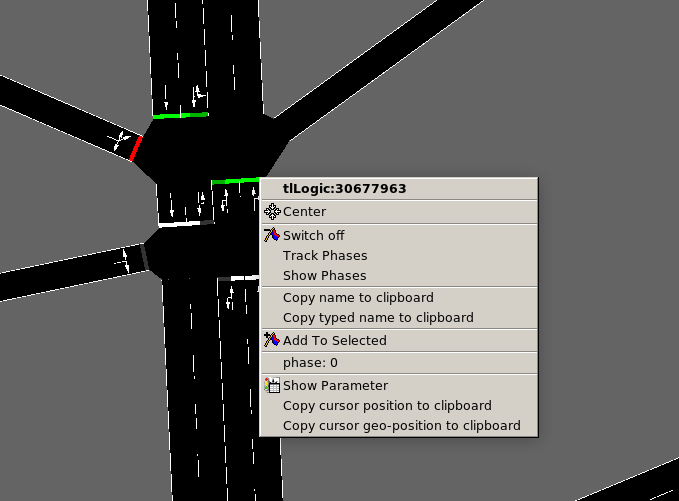
\includegraphics{./img/feux_sumo.png}
        \caption{Feux ~30677963~ à l'état ~GrG~ en partant du haut et en allant dans le sens anti-horaire.}
    \end{subfigure}%
    ~ 
    \begin{subfigure}[t]{0.5\textwidth}
        \centering
        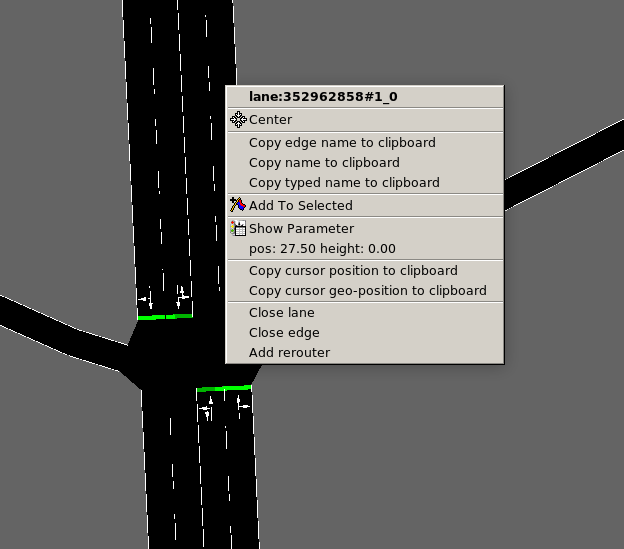
\includegraphics{./img/arrete_file_sumo.png}
        \caption{File ~1~ de l'arrête ~352962858#1~.}
    \end{subfigure}
    \caption{Nomenclature utilisée par Sumo.}
\end{figure*}
\end{latex}

\subsection{Sim4sys}
\label{sec:org9da9a76}

\subsection{Architectures logicielles}
\label{sec:org9c28fad}

Pour satisfaire les besoins métier tout en gardant l'état de l'art en matière d'infrastructure d'entraînement, nous avons choisi d'entraîner l'agent sur \emph{Sumo} via \emph{Flow} d'une part, et de l'interfacer avec le simulateur de production de CIL4SYS, \emph{Sim4sys} d'autre part. L'analyse des données TomTom sur Issy les Moulineaux a permis de déterminer une zone d'étude. L'import du terrain d'analyse dans Sumo s'effectue grâce à l'outil d'export d'\emph{Open Street Map} et la fonctionnalité d'import de carte fournie par \emph{Flow}.

Une fois l'agent entraîné, il sera « servi » par un serveur \emph{Flask} communiquant en Websocket via le module Python \texttt{asyncio}. Les repères utilisés pour la génération des états étant différents entre \emph{Sumo} et \emph{Sym4sys}, une transformation (qui reste à finaliser à ce jour) doit donc être réalisée lors de l'interaction entre l'agent et le simulateur de production.

Les figures \ref{fig:train_arch} et  \ref{fig:prod_arch} schématisent ces architectures.

\begin{figure}[htbp]
\centering
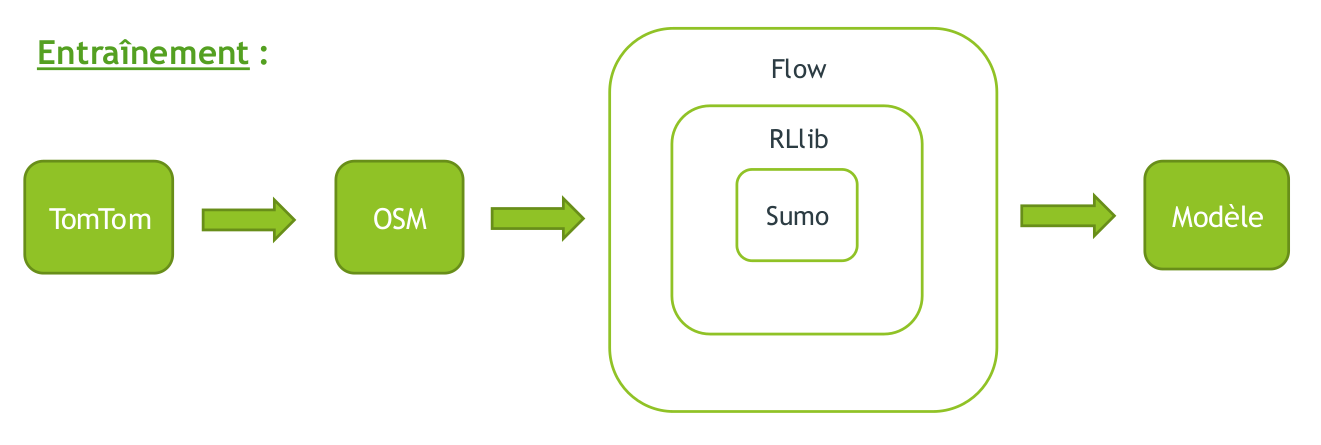
\includegraphics[width=.9\linewidth]{./img/entrainement_arch.png}
\caption{\label{fig:train_arch}
Architecture d'entraînement}
\end{figure}

\begin{figure}[htbp]
\centering
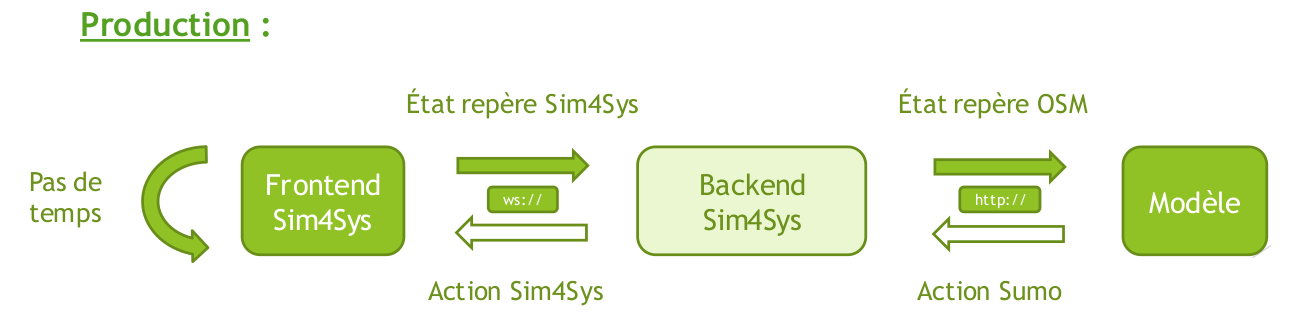
\includegraphics[width=.9\linewidth]{./img/production.png}
\caption{\label{fig:prod_arch}
Architecture de production}
\end{figure}

\section{Quartier d'étude}
\label{sec:orgf4a2322}

Le choix du quartier d'étude doit répondre à plusieurs contraintes : la présence de feux tricolores, un trafic qui ne soit pas trop dense comme l'est celui de Paris intra-muros, mais qui soit suffisamment congestionné pour que notre solution puisse apporter une amélioration.
En considération de la haute dimension de la formulation mathématique du problème, nous avons choisi d'étudier un ensemble de 4 intersections à Issy les Moulineaux, contrôlées par trois feux tricolores.

En effet, nous avons observé des congestions dans cette zone en période de pointe à l'aide de l'API TomTom et voudrions étudier si une solution par renforcement peut réduire ces bouchons.



\section{{\bfseries\sffamily TODO} Ajouter image}
\label{sec:orgd98edf9}

La figure \ref{fig:tomtom_data} bla bla bla.

\begin{figure}[htbp]
\centering
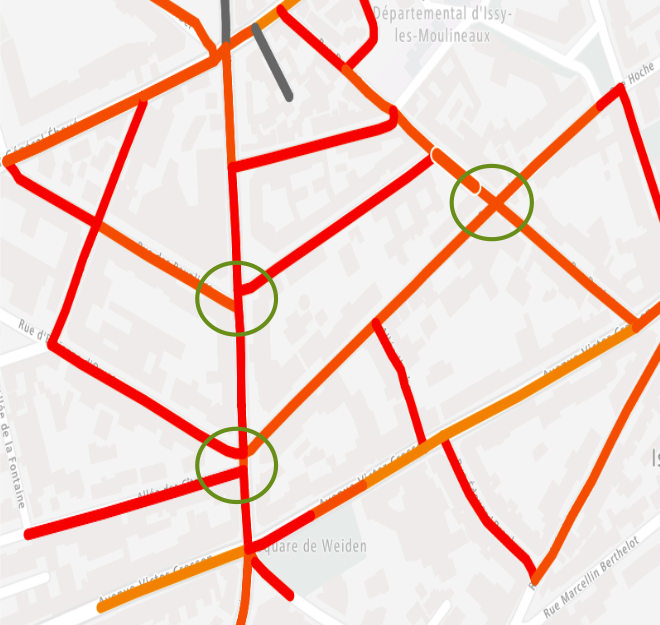
\includegraphics[width=200px]{./img/tomtom_data.png}
\caption{\label{fig:tomtom_data}
Les données de trafic TomTom sur le quartier séléctioné. Les intersections contrôlées par des feux sont encerclées en vert.}
\end{figure}


\section{{\bfseries\sffamily TODO} Ajouter justification}
\label{sec:orgfb99940}

\section{Modélisations}
\label{sec:org846459f}

Le DQN nous permettant de résoudre la formulation mathématique de notre problème en fonction d'un ensemble d'états, d'actions possibles sur ces états et d'une récompense entre ces transitions, il faut maintenant les définir.

\subsection{États}
\label{sec:orgf9273d9}

Dans une logique d'apprentissage, la question devient de trouver une représentation du système à un temps \(t\) qui encode toutes les informations nécessaires pour permettre de prendre \emph{la meilleure} action possible selon une certaine mesure qui reste à définir. Sans nécessairement formuler formellement à ce stade cette mesure, nous savons que le but de l'action prise est de fluidifier le trafic. Ainsi, nous aimerions donc que l'état encode des informations relatives à chaque véhicule simulé ainsi qu'aux feux tricolores.

Notre modèle d'état est donc une matrice composée de deux parties, l'une décrivant l'état des voitures, \(e^v\), et l'autre des feux, \(e^f\), à un pas de temps \(t\) donné:


\begin{latex}
\begin{equation}
    e = [e^v, e^f], \forall e \in \mathcal{E}
\end{equation}
\end{latex}

\subsubsection{Représentation des voitures observées, \(e^v\)}
\label{sec:org4ea00da}

En pratique l'algorithme de gestion des feux n'aura pas forcément la capacité de connaître l'état de tout les véhicules. Nous proposons donc un modèle où l'état d'apprentissage inclut seulement un sous ensemble de véhicules - envoyés par la mairie pour sonder le trafic par exemple, à l'aube des voitures électriques autonomes, cela semble tout à fait possible. Par ailleurs, la dimensionalité du problème d'étude s'en retrouve réduite.

Formellement, pour \(\beta\) voitures observées à chaque pas de temps \(t\), l'état \(e^v_i\) du \(i\) ème véhicule observé est décrit de la manière suivante :

\begin{latex}
\begin{equation}
    e^v_i = (x_i, y_i, \theta_i, v_i, \kappa_i, t^{v_0}_i) \subset \mathbb{R}^6 \mbox{ pour } i = 1, …, \beta
\end{equation}
\end{latex}

Où \(x_i, y_i, \theta_i, v_i, \kappa_i, t^{v_0}_i\) représentent l'ordonnée, l'abscisse, l'orientation, la vitesse absolue, le taux d'émission de \(CO_2\), et le temps passé à l'arrêt pour le \(i\) ème véhicule observé. En concaténant les \(i\) états, nous obtenons :

\begin{latex}
\begin{equation}
    e^v = [e^v_1, …, e^v_\beta] \subset \mathbb{R}^{6\times\beta}
\end{equation}
\end{latex}

\subsubsection{Représentation des feux, \(e^f\)}
\label{sec:org21f6848}

Contrairement à l'état des voitures, nous considérons que l'algorithme de gestion des feux a connaissance de l'état de l'ensemble des feux à synchroniser à chaque pas de temps. Bien que le quartier simulé n'ait que trois intersections contrôlées par des feux tricolores, il peut y avoir plus d'un feu par croisement. En effet, chaque file peut avoir un ou plusieurs feux en considérant les feux de type \emph{tourner à droite} ou \emph{U-turn}. En l'occurrence, le quartier d'analyse comporte 27 feux.

Par souci de simplicité, nous \textbf{restreignons} l'état de chaque feu à \emph{rouge} ou \emph{vert} et \textbf{ignorons} le \emph{orange}, cela consiste donc en une représentation binaire : \(e^f_i \in \{0,1\}\). Donc :

\begin{latex}
\begin{equation}
    e^f \in \{0,1\}^\gamma
\end{equation}
\end{latex}

\subsubsection{Représentation finale, \(e\in\mathcal{E}\)}
\label{sec:org48a6b6f}

Comme évoqué précédemment, l'état \(e = e^v + e^f\) de l'environnement à chaque instant \(t\) pour les \(\beta\) voitures observées et \(\gamma\) feux contrôlés est un élément de \(\mathcal{E}\subset \mathbb{R}^{6\times\beta}\times\{0,1\}^\gamma\).

\subsection{Actions}
\label{sec:org4c67f13}

Dans notre modèle, l'agent peut contrôler l'état de chacun des \(\gamma\) feux, chaque action \(a \in \mathcal{A}\) est donc un vecteur de \(\gamma\) booléens puisque seul les états \emph{rouge} et \emph{vert} sont considérés dans notre analyse.  Il y a donc \(2^\gamma\) actions possibles sur l'état des feux à chaque pas de temps. Le quartier comportant 27 feux, cela signifie qu'il y a un peu plus de 130 millions d'actions possibles sur le système à chaque pas de temps.

Il est donc nécessaire de choisir un sous ensemble d'actions, \(\mathcal{A}^* \subset \mathcal{A}\) de manière à réduire la dimensionalité de notre problème. Par ailleurs, certaines actions théoriquement possibles ne le sont pas en pratique, nous pensons notamment aux deux actions qui passent tous les feux au même état - ce qui au mieux immobiliserait tout le trafic et au pire serait catastrophique.

La cardinalité de \(\mathcal{A}^*\) ainsi que ses éléments est arbitraire bien que le but soit de trouver un « petit » ensemble d'actions qui « aient du sens » d'un point de vue de la gestion du trafic. Pour nous aider à la tâche, nous avons essayer de borner \(\mathcal{A^*}\) de la manière suivante: pour trois intersections contrôlées par des feux, il faudrait que chaque intersection ait au moins deux états. Alors, si \(n\) intersections sont contrôlées par \(\gamma \geq n\) feux, le nombre minimal d'actions pour que le modèle ait un sens est de \(2^n \leq \gamma^n\). Dans notre cas, pour \(n = 3\) et \(\gamma = 27\); nous avons donc \(|\mathcal{A}^*|\) bornées entre \(2^3\) et \(|\mathcal{A}| - 2 = 2^{27} - 2\) (le \(-2\) provenant des actions qui changent tous les feux au même état).

Pour commencer par le cas le plus simple, nous avons donc recensé deux états de feux par intersection en se demandant lesquelles permettraient de faire passer toutes les voitures à un moment ou à un autre. Les états sélectionnés sont exposés dans la structure de données du Listing \ref{code:tl_state_space}. Cette structure de données est un dictionnaire ayant pour clefs les chaîne de caractères identifiant les feux contrôlés et pour valeurs une liste de chaîne de caractères décrivant l'état des feux selon le format défini par Sumo. Son type est donc \texttt{OrderedDict< String, List<String> >}.

\begin{listing}[htbp]
\begin{minted}[]{python}
action_spec = OrderedDict({
    # The main traffic light, in sumo traffic light state strings
    # dictate the state of each traffic light and are ordered counter
    # clockwise.
    "30677963": [
        "GGGGrrrGGGG",  # allow all traffic on the main way w/ U-turns
        "rrrrGGGrrrr",  # allow only traffic from edge 4794817
    ],
    "30763263": [
        "GGGGGGGGGG",  # allow all traffic on main axis
        "rrrrrrrrrr",  # block all traffic on main axis to unclog elsewhere
    ],
    "30677810": [  # the smallest of all controlled traffic lights
        "GGrr",
        "rrGG",
    ],
})
\end{minted}
\caption{\label{code:tl_state_space}
Structure de données encodant les états de feux possibles du système.}
\end{listing}

Le fait que le dictionnaire soit ordonné permet de calculer le produit cartésien de ses clefs, qui représente l'ensemble des actions possibles privé de l'action identité, dans le même ordre à chaque pas de temps et donc de pouvoir associer les actions de l'agent à un nouvel état du système aisément, voir l'algorithme présenté sur le Listing \ref{code:take_rl_action}.

\begin{listing}[htbp]
\begin{minted}[]{python}
def map_action_to_tl_states(self, rl_actions):
    """Maps an rl_action list to new traffic light states based on
    `action_spec` or keeps current traffic light states as they are.

    Parameters
    ---------
    rl_actions: [float] list of action probabilities of cardinality
        `self.get_num_actions()`
    """
    identity_action = [
        tuple(
            self.k.traffic_light.get_state(id)
            for id in self.action_spec.keys())
    ]
    all_actions = list(itertools.product(
        *list(self.action_spec.values()))) + identity_action
    return all_actions[rl_actions]

\end{minted}
\caption{\label{code:take_rl_action}
Fonction d'association d'une action prise à nouvel état des feux : \(T : \mathcal{A}^* \longrightarrow \mathcal{E}^f\)}
\end{listing}

Nous retenons donc huit états de feux possibles et une action pour chacun d'entre eux. Cependant, nous avons choisi d'en inclure une neuvième, celle de l'action identité qui ne modifie pas l'état des feux. \emph{En effet, nous émettons l'hypothèse que l'agent apprendra plus vite laquelle des neuf actions ne modifie pas l'état plutôt que laquelle des huit actions faut il prendre à un état donné pour ne pas le modifier}. Nous obtenons donc finalement \(|\mathcal{A}^*| = 9\).

\subsection{Récompenses}
\label{sec:orgfa6677c}

Les états et actions du modèle étant maintenant définis, nous pouvons concevoir les fonctions de récompenses, l'idée étant guider l'agent durant l'apprentissage. Cependant, contrairement à une approche par optimisation sous contraintes, choisir une action de manière à maximiser l'espérance de la récompense ne garantit pas une solution contrainte. Par exemple, si la fonction de récompense pénalise les changements de feux trop fréquents mais récompense autre chose, alors l'agent évitera les changements trop fréquents, \emph{mais ne les excluera pas de la solution}. L'agent pourra par exemple choisir de changer l'état des feux à faibles intervalles occasionnellement si cela maximise l'espérance de la récompense à cet état donné. Une solution apprise par renforcement se comporte donc différemment qu'une solution à un problème d'optimisation sous contrainte « équivalent ». Nous verrons comment pallier à ce problème ultérieurement et nous focalisons maintenant sur la conception de fonctions de récompenses pertinentes.

Nous voudrions concevoir une fonction de récompense qui encourage :

\begin{itemize}
\item le débit des flux
\item les voitures en mouvement
\end{itemize}

Et pénalise :

\begin{itemize}
\item les accélérations
\item les émissions de \(CO_2\)
\item les changements de feux
\item les voitures arrêtées pendant trop longtemps
\end{itemize}

Une fonction de récompense simple est par exemple :

$$\psi = \frac{\bar{v}}{\bar{\kappa}}$$

Où \(\bar{v}\) et \(\bar{\kappa}\) représentent la vitesse moyenne et le taux d'émission moyen des \(\beta\) véhicules observés par l'agent. Le but de cette fonction est de favoriser le débit tout en minimisant les émissions. Cependant, cette fonction est naïve et inadaptée à notre problème puisque la solution serait de laisser l'artère avec le débit de véhicules le plus important et de bloquer tous les autres. Il faudrait donc pouvoir intégrer d'autres variables à la fonction de récompense. L'image de cette fonction étant un sous ensemble de \(\mathbb{R}\), ces différentes composantes ne peuvent être qu'additionnées entre elles. Cependant la fonction suivante n'a pas de sens :

$$\psi = C_1\bar{v} - C_2\bar{\kappa} - C_3\bar{t}^{v_0}$$

Où les \(C_i\) sont des constantes et \(\bar{t^{v_0}}\) la moyenne d'une mesure de temps passé à l'arrêt par les voitures. En effet, le dimensionnement des constantes est très délicat puisque leurs unités sont incompatibles entre elles et ne peuvent être additionnées.

Une façon plus simple de composer la fonction de récompense et de définir un certain nombre de contraintes sur l'état des voitures et de compter les véhicules sous ou sur telle ou telle contrainte. Par exemple, une fonction qui récompense les voitures allant à une vitesse supérieure à \(v_{min}\) sera définie de la manière suivante :

$$\psi = \sum^{\beta}_{i=1}\mathbb{I}\{v_i \geq v_{min}\}$$

Cette manière de construire la récompense permet de composer ses termes. La composante due à l'état des voitures de la récompense de notre modèle, \(\psi^v\) est la suivante:

\begin{latex}
\begin{equation}
  \psi^v = \sum^{\beta}_{i=1}\left[
    C_1 \cdot \mathbb{I}\{v_i \geq v_{min}\}
    - C_2 \cdot \mathbb{I}\{\kappa_i \geq \kappa_{min}\}
    - C_3 \cdot \mathbb{I}\{t^{v_0}_i \geq \tau\}
  \right]
\end{equation}
\end{latex}

Par ailleurs, pour inciter l'agent à ne changer l'état des feux que lorsqu'il « a beaucoup à gagner », nous incorporons une composante pénalisant les changements de feux :

\begin{latex}
\begin{equation}
  \psi^f = \sum^{\gamma}_{i=1}\left[
    C_4 \cdot \mathbb{I}\{e^f_{i, t} \neq e^f_{i, t-1}\}
  \right]
\end{equation}
\end{latex}

Où \(e^f_{i, t}\) est l'état du feu \(i\) à l'instant \(t\). Nous obtenons alors la récompense de notre modèle aisément:

\begin{latex}
\begin{equation}
  \psi = \psi^e + \psi^f
\end{equation}
\end{latex}

Cette fonction de récompense dépend donc de l'état du système au temps \(t\) mais aussi à quatre constantes, « hyperparamètres » en un sens, à accorder à la main pour le moment. En effet, valider une solution revient à la visualiser puis à la valider qualitativement à ce stade. Nous n'avons pas encore de méthode automatisable pour réaliser cela, les quatre constantes doivent donc être ajustées \emph{manuellement}.

\subsection{Environments de simulations}
\label{sec:orgad5e055}

\subsection{Notes d'implémentation}
\label{sec:org99bcd80}

\section{Infrastructure de calcul}
\label{sec:orgc23a640}

\subsection{Colab}
\label{sec:orga21e5a5}

\subsection{Cluster de machines de TP}
\label{sec:orge8bbcef}

\subsection{Serveur AWS}
\label{sec:org5bd790f}

\section{Méthode de validation des solutions}
\label{sec:org2264e28}


\section{Résultats}
\label{sec:org733056c}


\section{Conclusion}
\label{sec:org470be2a}
\end{document}
